% ===========================================================================
\section{Milestone III: Evolution of the perturbations}\label{sec:m3}
% ===========================================================================

The Universe is not perfectly homogeneous. The CMB temperature varies across the sky at the level of $10^{-5}$, and
these tiny primordial fluctuations have grown into the galaxies and clusters we see today. The third milestone follows
the fluctuations from the radiation era until today. Since they are small, we expand Einstein's equations and the
Boltzmann equations for every species to first order around the FLRW background of Milestone~I. The background is
translation invariant, so in Fourier space each wavenumber evolves independently, and isotropy means that only the
magnitude $k$ matters. The output is a set of transfer functions and source functions that the line-of-sight
integration of Milestone~IV turns into the observed spectra.

\subsection{Theory}

\paragraph*{The perturbed metric.} We work in the conformal Newtonian gauge,
\begin{equation}
\dd s^2 = a^2(\eta)\big[-(1+2\Psi)c^2\dd\eta^2 + (1+2\Phi)\delta_{ij}\dd x^i\dd x^j\big],
\end{equation}
with the variables and sign conventions of Callin~\cite{Callin2006}, which follow Dodelson~\cite{Dodelson2003}. $\Psi$
plays the role of the Newtonian gravitational potential: it governs the motion of non-relativistic particles and the
redshift of light climbing out of a potential well. $\Phi$ is a perturbation of the spatial curvature, so a changing
$\Phi$ stretches space locally and redshifts photons in the same way the background expansion does. In the absence of
anisotropic stress the two are equal and opposite, $\Psi=-\Phi$.

We write $\kappa\equiv ck/\Hp$, the wavenumber in units of the comoving Hubble scale. A mode is outside the horizon when
$\kappa\ll1$ and inside when $\kappa\gg1$; most of the interesting physics happens at horizon entry, $\kappa\approx1$.

\paragraph*{The Boltzmann equation for photons.} The photon distribution function is a Planck spectrum with a
direction-dependent temperature, $f=[\exp(p/k_BT(1+\Theta))-1]^{-1}$, where the fractional temperature perturbation
$\Theta(\bm{x},\hat{\bm p},\eta)$ depends on position and on the direction of the photon momentum. In Fourier space
$\Theta$ depends on $k$ and on $\mu=\hat{\bm k}\cdot\hat{\bm p}$. The linearized Boltzmann equation
$\dd f/\dd\eta=C[f]$ becomes
\begin{align}
\Theta' + i\kappa\mu\Theta &= -\Phi' - i\kappa\mu\Psi \nonumber\\
 &\quad - \tau'\Big[\Theta_0 - \Theta + i\mu v_b - \tfrac12P_2(\mu)\Pi\Big].
\label{eq:boltz_photon}
\end{align}
Each term has a clear physical meaning:
\begin{itemize}
\item $i\kappa\mu\Theta$ is free streaming. Photons move in direction $\hat{\bm p}$, so an inhomogeneity in space turns
      into an anisotropy in direction.
\item $-\Phi'$ is the redshift caused by the local change of spatial curvature.
\item $-i\kappa\mu\Psi$ is the gravitational redshift (or blueshift) of photons that climb out of (or fall into) a
      potential gradient.
\item The last term is Thomson scattering, at rate $-\tau'$ per unit $x$. Scattering drives the distribution towards
      isotropy, $\Theta\to\Theta_0$. Electrons moving with velocity $v_b$ Doppler shift the scattered photons, which
      gives the $\mu v_b$ term. Thomson scattering is not isotropic but goes as $1+\cos^2$ of the scattering angle, which
      gives the quadrupole term $P_2\Pi$.
\end{itemize}
We expand in Legendre polynomials,
$\Theta_\ell=\frac{1}{(-i)^\ell}\int_{-1}^1\frac{\dd\mu}{2}P_\ell(\mu)\Theta(\mu)$, and the low multipoles are the familiar
fluid quantities:
\begin{itemize}
\item the monopole $\Theta_0$ gives the density, $\delta_\gamma=4\Theta_0$ since $\rho_\gamma\propto T^4$;
\item the dipole gives the velocity, $v_\gamma=-3\Theta_1$;
\item the quadrupole $\Theta_2$ is the anisotropic stress.
\end{itemize}
Multiplying Eq.~\eqref{eq:boltz_photon} by $P_\ell$ and integrating, the $\mu\Theta$ term couples each $\ell$ to
$\ell\pm1$, because $\mu P_\ell$ is a combination of $P_{\ell-1}$ and $P_{\ell+1}$. This gives the hierarchy
\begin{align}
\Theta_0' &= -\kappa\Theta_1 - \Phi', \\
\Theta_1' &= \frac{\kappa}{3}(\Theta_0 - 2\Theta_2 + \Psi) + \tau'\Big(\Theta_1 + \frac{v_b}{3}\Big), \\
\Theta_\ell' &= \frac{\kappa\big[\ell\Theta_{\ell-1} - (\ell+1)\Theta_{\ell+1}\big]}{2\ell+1}
               + \tau'\Big(\Theta_\ell - \frac{\Pi}{10}\delta_{\ell2}\Big),
\end{align}
where the factors of $i$ have been absorbed into the definition of the velocities. The monopole equation is the
continuity equation of the photon fluid, and the dipole equation is its Euler equation. Free streaming moves power from
low to high $\ell$: an inhomogeneity on scale $1/k$ viewed from a distance $d$ appears as an anisotropy at
$\ell\sim kd$. Scattering instead damps all $\ell\ge2$ multipoles and locks $\Theta_1$ to the baryon velocity.

\paragraph*{Polarization.} Thomson scattering of radiation with a quadrupole anisotropy produces linearly polarized
light: the scattered wave is polarized perpendicular to the plane of scattering, and an incoming quadrupole makes
the polarization from different directions not cancel. Its multipoles $\Theta^P_\ell$ obey a similar
hierarchy~\cite{Zaldarriaga1995}, sourced by $\Pi=\Theta_2+\Theta^P_0+\Theta^P_2$:
\begin{align}
\Theta^{P\prime}_\ell &= \frac{\kappa\big[\ell\Theta^P_{\ell-1} - (\ell+1)\Theta^P_{\ell+1}\big]}{2\ell+1} \nonumber\\
      &\quad + \tau'\Big[\Theta^P_\ell - \frac{\Pi}{2}\Big(\delta_{\ell0}+\frac{\delta_{\ell2}}{5}\Big)\Big].
\end{align}
Polarization has no gravitational source: it is created only by scattering of a quadrupole.

\paragraph*{Neutrinos.} Neutrinos decoupled long before the earliest time we consider, so their Boltzmann equation is
Eq.~\eqref{eq:boltz_photon} without the collision term. Their multipoles $\mathcal{N}_\ell$ obey the photon hierarchy
with $\tau'=0$. Massless neutrinos therefore free-stream from the start. Their quadrupole $\mathcal{N}_2$ is a large
anisotropic stress during the radiation era, when they make up $41\%$ of the radiation density.

\paragraph*{Dark matter and baryons.} Cold dark matter is collisionless and non-relativistic. The first two moments of
its Boltzmann equation (equivalently, energy--momentum conservation) are the continuity and Euler equations,
\begin{equation}
\delta_{\rm CDM}' = \kappa v_{\rm CDM} - 3\Phi', \qquad v_{\rm CDM}' = -v_{\rm CDM} - \kappa\Psi.
\end{equation}
In the continuity equation $\kappa v$ is the inflow of matter, and $-3\Phi'$ the change of the local volume when the
spatial metric is perturbed. In the Euler equation $-v$ is the Hubble drag, which redshifts peculiar momenta as
$a^{-1}$, and $-\kappa\Psi$ is the gravitational force. Baryons obey the same equations plus the momentum they
exchange with the photons through Thomson scattering:
\begin{align}
\delta_b' &= \kappa v_b - 3\Phi', \\
v_b' &= -v_b - \kappa\Psi + \tau'R(3\Theta_1+v_b).
\end{align}
The factor $R=4\rho_\gamma/3\rho_b$ ensures momentum conservation. The momentum the photons lose (the $\tau'$ term in
the $\Theta_1$ equation) is gained by the baryons, whose momentum density is smaller by $\rho_b/(\tfrac43\rho_\gamma)$.

\paragraph*{Einstein equations.} The perturbed Einstein equations relate the potentials to the matter. The $00$
component, together with the $0i$ component, gives
\begin{align}
\Phi' &= \Psi - \frac{\kappa^2}{3}\Phi + \frac{H_0^2}{2\Hp^2}\Big[\frac{\Om_{\rm CDM}\delta_{\rm CDM}+\Om_b\delta_b}{a} \nonumber\\
      &\qquad + \frac{4(\Om_\gamma\Theta_0+\Om_\nu\mathcal{N}_0)}{a^2}\Big], \label{eq:einstein1}
\end{align}
where $\Om_i$ are today's values. Deep inside the horizon ($\kappa\gg1$) this reduces to the Poisson equation,
$k^2\Phi\propto a^2\delta\rho$. The traceless part of the $ij$ components gives
\begin{equation}
\Psi = -\Phi - \frac{12H_0^2}{c^2k^2a^2}\big[\Om_\gamma\Theta_2+\Om_\nu\mathcal{N}_2\big],
\label{eq:einstein2}
\end{equation}
so $\Psi\neq-\Phi$ only if there is anisotropic stress: the quadrupoles of the photons and neutrinos.

\paragraph*{Truncation.} We truncate the hierarchies at $\ell_{\max}$ with the closure of Ma \&
Bertschinger~\cite{Ma1995}. It assumes the free-streaming solution $\Theta_\ell\propto j_\ell(k\eta)$ for the highest
multipole, to avoid an artificial reflection of power back down to low $\ell$:
\begin{equation}
\Theta_{\ell_{\max}}' = \kappa\Theta_{\ell_{\max}-1} - \frac{c(\ell_{\max}+1)}{\Hp\eta}\Theta_{\ell_{\max}}
+\tau'\Theta_{\ell_{\max}}.
\end{equation}

\paragraph*{Initial conditions.} At $x=-18$ every mode is far outside the horizon ($\kappa\ll1$) and the Universe is
radiation dominated. Inflation produces \emph{adiabatic} fluctuations: the whole Universe is locally the same, but
slightly ahead of or behind in time. Then the number densities of all species are perturbed equally,
$\delta_{\rm CDM}=\delta_b=\tfrac34\delta_\gamma=\tfrac34\delta_\nu$. Solving the equations to lowest order in $\kappa$
gives $\Phi'=0$ and $\Theta_0=-\Psi/2$. The neutrino quadrupole in Eq.~\eqref{eq:einstein2} gives
$\Phi=-(1+2f_\nu/5)\Psi$, with $f_\nu=\Om_\nu/(\Om_\gamma+\Om_\nu)$. We normalize to a primordial comoving curvature
perturbation $\mathcal{R}=1$, which is conserved outside the horizon and is the quantity inflation predicts. Then
\begin{align}
\Psi &= -\frac{1}{\tfrac32+\tfrac25f_\nu}, \quad \Phi = -\Big(1+\frac{2f_\nu}{5}\Big)\Psi, \nonumber\\
\delta_{\rm CDM} &=\delta_b=-\frac32\Psi,\quad v_{\rm CDM} = v_b = -\frac{\kappa}{2}\Psi, \nonumber\\
\Theta_0 &=\mathcal{N}_0=-\frac{\Psi}{2},\quad \Theta_1=\mathcal{N}_1=\frac{\kappa}{6}\Psi, \nonumber\\
\mathcal{N}_2 &= -\frac{(cka)^2\Phi}{12H_0^2\Om_\nu}\Big(1+\frac{5}{2f_\nu}\Big)^{-1},
\end{align}
and $\mathcal{N}_\ell=\kappa\mathcal{N}_{\ell-1}/(2\ell+1)$ for $\ell\ge3$. The actual amplitude of each mode is
restored in Milestone~IV through the primordial power spectrum $\mathcal{P}_{\mathcal{R}}(k)$.

\paragraph*{Tight coupling and acoustic oscillations.} At early times $|\tau'|\gg1$: a photon scatters thousands of
times per Hubble time. The scattering terms force $\Theta_1\simeq-v_b/3$, and the photon multipoles with $\ell\ge2$ are
suppressed by powers of $\kappa/\tau'$. The photons and baryons then behave as one fluid. Combining the $\Theta_0$,
$\Theta_1$ and $v_b$ equations at leading order in $1/\tau'$ gives, in conformal time,
\begin{align}
\frac{\dd}{\dd\eta}\Big[(1+R_b)\dot\Theta_0\Big] + \frac{c^2k^2}{3}\Theta_0
 &= -\frac{c^2k^2}{3}(1+R_b)\Psi \nonumber\\
 &\quad - \frac{\dd}{\dd\eta}\Big[(1+R_b)\dot\Phi\Big],
\label{eq:oscillator}
\end{align}
with $R_b=1/R=3\rho_b/4\rho_\gamma$. This is a driven harmonic oscillator. Photon pressure provides the restoring force,
baryons add inertia ($1+R_b$) and lower the sound speed to $c_s=c/\sqrt{3(1+R_b)}$, and gravity drives it. For slowly
varying potentials and $R_b$ the adiabatic solution is
\begin{equation}
\Theta_0+(1+R_b)\Psi \simeq A\cos(kr_s),
\label{eq:acoustic}
\end{equation}
where $r_s$ is the sound horizon of Milestone~II. These are the acoustic oscillations of the photon--baryon fluid. Two
features are important for the CMB:
\begin{itemize}
\item The observed temperature includes the gravitational redshift, $\Theta_0+\Psi=A\cos(kr_s)-R_b\Psi$. Baryons shift
      the zero point of the oscillation, so compressions in potential wells are enhanced relative to rarefactions.
\item When a mode enters the horizon in RD, the potentials decay just as the fluid is first compressed. The decay
      removes the gravitational pull that would otherwise slow the rebound, which boosts the oscillation amplitude
      (``radiation driving'').
\end{itemize}

At next order in $1/\tau'$ photons diffuse over their mean free path and smooth out the oscillations (Silk damping):
$\Theta_0\propto e^{-k^2/k_D^2}$ with~\cite{HuSugiyama1995}
\begin{equation}
k_D^{-2} = \int_0^\eta \frac{c\,\dd\eta'}{6(1+R_b)\,n_e\sigma_Ta}\Big[\frac{R_b^2}{1+R_b}+\frac{16}{15}\Big].
\label{eq:silk}
\end{equation}
This is a random walk: the diffusion length is the geometric mean of the mean free path and the horizon.

Numerically, the tight-coupling regime is too stiff to integrate the full hierarchy. We evolve only
$\delta_{\rm CDM},v_{\rm CDM},\delta_b,v_b,\Phi,\Theta_0,\Theta_1$ (and the neutrinos), and set
\begin{equation}
\Theta_2 = -\frac{8}{15}\frac{\kappa}{\tau'}\Theta_1, \quad \Theta^P_0=\frac54\Theta_2, \quad \Theta^P_2=\frac14\Theta_2,
\end{equation}
with $\Theta_\ell=-\frac{\ell}{2\ell+1}\frac{\kappa}{\tau'}\Theta_{\ell-1}$ for $\ell\ge3$ (and the same for
$\Theta^P$). These are the quasi-static solutions of the hierarchy when the $\tau'$ terms dominate. Without polarization,
$8/15$ becomes $20/45$. Polarization feeds back on $\Theta_2$ through $\Pi$, which raises the quadrupole by a factor
$6/5$. The baryon velocity and $\Theta_1$ follow from the second-order expansion of Ref.~\cite{Callin2006}, which
eliminates the large $\tau'$ terms in favour of the slip $q\equiv3\Theta_1'+v_b'$:
\begin{align}
q &= \Big\{-[(1-R)\tau'+(1+R)\tau'']\,(3\Theta_1+v_b) - \kappa\Psi \nonumber\\
  &\qquad + \Big(1-\frac{\Hp'}{\Hp}\Big)\kappa(-\Theta_0+2\Theta_2) - \kappa\Theta_0'\Big\} \nonumber\\
  &\quad \Big/\Big[(1+R)\tau'+\frac{\Hp'}{\Hp}-1\Big], \nonumber\\
v_b' &= \frac{-v_b - \kappa\Psi + R\big[q + \kappa(-\Theta_0+2\Theta_2) - \kappa\Psi\big]}{1+R}, \nonumber\\
\Theta_1' &= \frac{1}{3}(q - v_b').
\end{align}
Tight coupling ends when $|\tau'|<10$, when $|\kappa/\tau'|>0.1$, or at $z=1700$ (before recombination starts),
whichever comes first.

\paragraph*{Analytic limits.} A few exact results guide the interpretation and serve as tests:
\begin{itemize}
\item Outside the horizon $\Phi$ is constant within each era. Through radiation--matter equality it drops by the factor
      $9/10$ (without neutrinos). With $\mathcal{R}=1$, $\Phi=3/5$ in MD. The full superhorizon solution through
      equality is known analytically~\cite{Kodama1984}.
\item Inside the horizon in RD, the potential obeys $\Phi=3\Phi_0(\sin y-y\cos y)/y^3$ with $y=k\eta/\sqrt3$. It
      oscillates and decays as $a^{-2}$, because radiation pressure prevents the density contrast from growing while
      the background density falls as $a^{-4}$.
\item In MD $\Phi$ is constant on all scales: $\delta\propto a$ and $\rho_Ma^2\propto a^{-1}$ cancel in the Poisson
      equation. In the $\Lambda$ era $\Phi\propto D(a)/a$ decays, where $D$ is the linear growth factor.
\item Sub-horizon dark matter obeys $\ddot\delta+2H\dot\delta=4\pi G\rho_M\delta$ (ignoring the radiation
      perturbations). In RD the source is negligible and $\delta\propto\ln a$ (the M\'esz\'aros effect). In MD
      $\delta\propto a$. In general the growth rate is $f=\dd\ln\delta/\dd\ln a\approx\Om_M(x)^{0.55}$.
\end{itemize}

\paragraph*{Source functions.} After the evolution we build the temperature and $E$-mode source functions:
\begin{align}
S_T(k,x) &= \gt\Big[\Theta_0+\Psi+\frac{\Pi}{4}\Big] + e^{-\tau}(\Psi'-\Phi') \nonumber\\
 &\quad - \frac{1}{ck}\frac{\dd}{\dd x}(\Hp\gt v_b)
  + \frac{3}{4c^2k^2}\frac{\dd}{\dd x}\Big[\Hp\frac{\dd}{\dd x}(\Hp\gt\Pi)\Big], \label{eq:ST}\\
S_E(k,x) &= \frac{3\gt\,\Pi}{4k^2(\eta_0-\eta)^2}. \label{eq:SE}
\end{align}
They come from integrating Eq.~\eqref{eq:boltz_photon} along the line of sight (Sec.~\ref{sec:m4}); the derivatives
arise from integrating the $\mu$-dependent terms by parts. They express the temperature we see as a sum over all
places where a photon last scattered (weighted by $\gt$) or was redshifted on its way (weighted by $e^{-\tau}$). The
four terms are, in order:
\begin{itemize}
\item the Sachs--Wolfe (SW) term: the intrinsic temperature at last scattering plus the gravitational redshift out of
      the potential well there;
\item the integrated Sachs--Wolfe (ISW) term: the net energy change of a photon crossing a time-varying potential;
\item the Doppler term: from the velocity of the electrons that last scattered the photon;
\item a small correction from the anisotropic, polarization-dependent nature of Thomson scattering.
\end{itemize}

\subsection{Implementation and tests}

\texttt{Perturbations} solves 400 modes, logarithmically spaced in $k\in[5\times10^{-5},0.3]\Mpc^{-1}$, on a
non-uniform grid of 2100 points in $x\in[-18,0]$ that is dense around recombination. The modes run in parallel with
OpenMP. We keep $\ell_{\max}=8$ for $\Theta_\ell$ and $\Theta^P_\ell$, and $\ell_{\max,\nu}=22$ for the neutrinos;
going to $\ell_{\max,\nu}=30$ changes the spectra by less than $5\times10^{-4}$. Only the low photon multipoles enter
the sources, so a small $\ell_{\max}$ is enough. The tight-coupling system is solved with an explicit Runge--Kutta
method (RK8PD). The full system is stiff, because $|\tau'|$ is still large when tight coupling ends, so we use the
implicit BDF method of GSL with a finite-difference Jacobian. The relative tolerance is $10^{-8}$. At the switch we
initialize the full hierarchy from the tight-coupling expressions above. The derivatives in $S_T$ come from splines in
$x$, and all quantities are stored as 2D bicubic splines in $(x,k)$.

The tests (Fig.~\ref{fig:m3_tests} and the unit tests) check the analytic limits listed above:
\begin{itemize}
\item On superhorizon scales the solution matches the exact Kodama--Sasaki solution through equality, and
      $\Phi\to3/5$ in MD.
\item For modes that enter in RD, $\Phi$ follows the analytic radiation-era solution until equality approaches
      (middle panel).
\item Before decoupling, $\Theta_0+\Psi$ oscillates as $\cos(kr_s)$, with the phase given by the sound horizon of
      Milestone~II (left panel). This tests the sound speed, and with it $R$.
\item In matter and $\Lambda$ domination the growth rate $\dd\ln\delta_{\rm CDM}/\dd x$ of small-scale modes follows
      $\Om_M(x)^{0.55}$ (right panel).
\end{itemize}
In addition, the Poisson equation holds on subhorizon scales today, the tight-coupling and full solutions are
continuous at the switch, and the neutrino multipoles free-stream as expected. All perturbations agree with CLASS to
$\sim0.1\%$.

\begin{figure*}
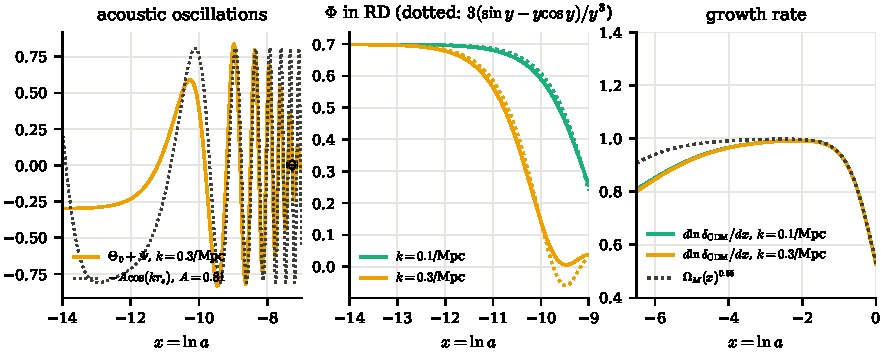
\includegraphics[width=\textwidth]{m3_tests}
\caption{Tests of the perturbations. \emph{Left:} $\Theta_0+\Psi$ for $k=0.3\Mpc^{-1}$ during the radiation era
compared with $-A\cos(kr_s)$, using the sound horizon $r_s$ from Milestone~II. After horizon entry the decaying
potential drives the oscillator, so the amplitude $A$ is fitted; the test is the phase. \emph{Middle:} $\Phi$ for
modes that enter in RD, compared with the analytic radiation-era solution (dotted). \emph{Right:} the growth rate of
$\delta_{\rm CDM}$ compared with $\Om_M(x)^{0.55}$.}
\label{fig:m3_tests}
\end{figure*}

\subsection{Results}

We show four modes, chosen to probe the different regimes:
\begin{itemize}
\item $k=0.001\Mpc^{-1}$ enters the horizon ($\kappa=1$) at $x=-4.13$ ($z\approx61$), well into MD. It is
      outside the horizon at recombination and probes the largest scales in the CMB.
\item $k=0.01\Mpc^{-1}$ enters at $x=-8.08$, close to equality.
\item $k=0.1\Mpc^{-1}$ enters at $x=-10.71$ and $k=0.3\Mpc^{-1}$ at $x=-11.83$, both deep in RD. They oscillate many
      times before recombination.
\end{itemize}
Tight coupling ends at $x=-7.44$ ($z=1700$) for the first three modes, and at $x=-7.89$ for $k=0.3\Mpc^{-1}$, where
$\kappa/\tau'$ becomes large first. Horizon entry is marked by coloured dotted lines in the figures, and grey lines mark
radiation--matter equality and decoupling.

\begin{figure*}
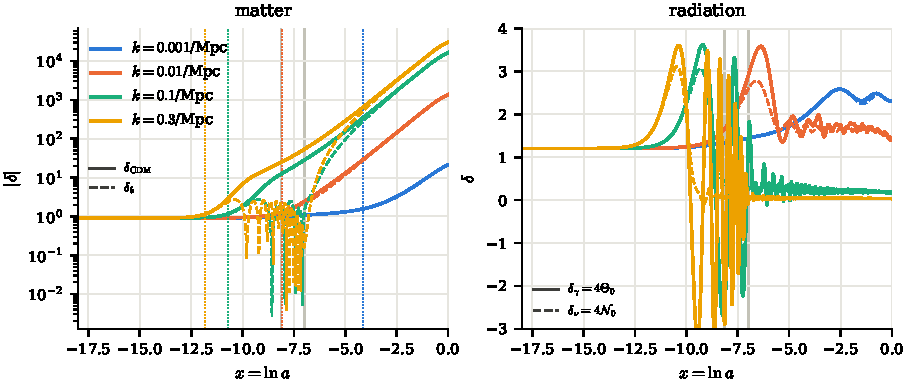
\includegraphics[width=\textwidth]{m3_delta}
\caption{Density perturbations. \emph{Left:} $|\delta_{\rm CDM}|$ (solid) and $|\delta_b|$ (dashed). The coloured
dotted lines mark horizon entry of each mode. \emph{Right:} photon $\delta_\gamma=4\Theta_0$ (solid) and neutrino
$\delta_\nu=4\mathcal{N}_0$ (dashed). Grey lines mark radiation--matter equality and decoupling ($\tau=1$).}
\label{fig:delta}
\end{figure*}

\begin{figure*}
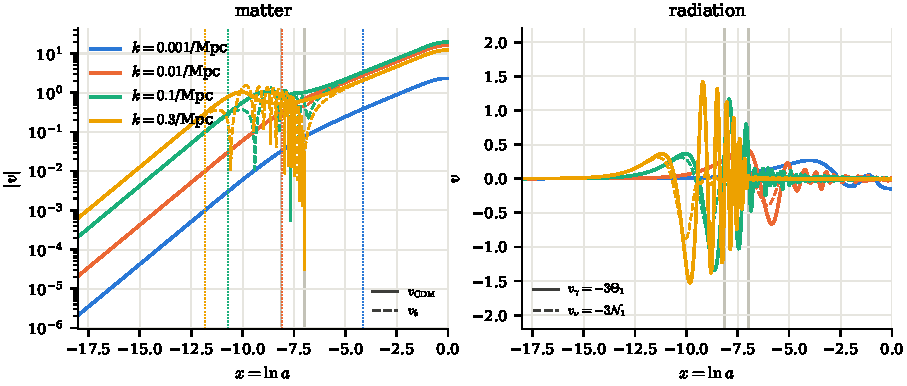
\includegraphics[width=\textwidth]{m3_velocity}
\caption{Velocities. \emph{Left:} $|v_{\rm CDM}|$ (solid) and $|v_b|$ (dashed). \emph{Right:} photon
$v_\gamma=-3\Theta_1$ (solid) and neutrino $v_\nu=-3\mathcal{N}_1$ (dashed).}
\label{fig:velocity}
\end{figure*}

\paragraph*{Dark matter.} Figure~\ref{fig:delta} shows the density contrasts. Outside the horizon all $\delta$'s are
nearly constant at $\delta=-\frac32\Psi$. There is no causal mechanism to change them, and in our gauge the
superhorizon density contrast only changes through the changing potential at equality. After horizon entry the
behaviour of $\delta_{\rm CDM}$ depends on when the mode entered:
\begin{itemize}
\item Modes that enter in RD ($k=0.1$, $0.3\Mpc^{-1}$) receive a kick from the decaying potential at horizon entry.
      After that they grow only slowly, because the dark matter's self-gravity is negligible compared with the
      expansion driven by the smooth radiation. The dark matter coasts on the velocity it got at entry, and
      $\delta_{\rm CDM}$ grows logarithmically (the M\'esz\'aros effect).
\item After equality, matter dominates gravity and all modes grow as $\delta_{\rm CDM}\propto a$.
\item In the $\Lambda$ era growth slows down (Fig.~\ref{fig:m3_tests}, right). For $k=0.1\Mpc^{-1}$, $\delta_{\rm CDM}$
      grows by a factor 107 from $x=-5$ to today, instead of $e^5=148$ for $\delta\propto a$.
\item The mode $k=0.001\Mpc^{-1}$ starts to grow as it approaches horizon entry in MD and has not reached the
      $\delta\propto a$ regime until late.
\end{itemize}
Small scales enter earlier and spend more time inside the horizon, but the time they spend in RD is lost to the
M\'esz\'aros stagnation. This suppression of modes with $k>k_{\rm eq}$ is the origin of the turnover in $P(k)$
(Sec.~\ref{sec:m4}).

\paragraph*{Baryons.} As long as they are tightly coupled to the photons, the baryons share the photon acoustic
oscillations, and adiabaticity gives $\delta_b\simeq\frac34\delta_\gamma$. Their density contrast is stuck at the photon
level, while $\delta_{\rm CDM}$ already grows. After decoupling the baryons lose the photon pressure and fall into the
potential wells that the dark matter has built. In MD the solution is $\delta_b\simeq\delta_{\rm CDM}(1-a_d/a)$, so
within a few $e$-folds $\delta_b$ catches up. For $k=0.1\Mpc^{-1}$, $\delta_b/\delta_{\rm CDM}$ goes from $0.04$ at
$x=-7$ to $0.29$ at $x=-6$ and $0.93$ at $x=-3$; today they are equal to within $0.5\%$. The remaining difference is the
acoustic imprint, the BAO. Without dark matter the baryon perturbations would have had to grow from their value at
decoupling, $\delta_b\sim10^{-5}\times$ (a few), by only the factor $\sim10^3$ available since recombination. That is
not enough to form galaxies. Dark matter is needed to give structure a head start.

\paragraph*{Photons and neutrinos.} The photons (Fig.~\ref{fig:delta}, right) oscillate after horizon entry: these
are the acoustic oscillations of Eq.~\eqref{eq:acoustic}. The amplitude grows at horizon entry because of radiation
driving, and the oscillation is offset from zero by the baryon loading term $-R_b\Psi$. Diffusion then damps the
oscillation. At decoupling $k_D\approx0.14\Mpc^{-1}$ (Eq.~\ref{eq:silk}), so the $k=0.3\Mpc^{-1}$ mode has lost most
of its amplitude: $|\Theta_0+\Psi|$ drops from $0.84$ at $x\approx-9$ to $0.2$ at decoupling. The $k=0.1\Mpc^{-1}$ mode
is only mildly damped. After decoupling the photons free-stream, $\Theta_0$ decays, and the power moves to higher
multipoles; at late times $\Theta_0\approx-\Psi$, so that the observed
$\Theta_0+\Psi$ averages to zero inside the horizon.

The neutrinos have been free-streaming all along. They have no pressure that can restore an acoustic oscillation, so
$\delta_\nu$ oscillates with decaying amplitude like a Bessel function as soon as the mode enters the horizon.

\paragraph*{Velocities.} The velocities (Fig.~\ref{fig:velocity}) tell the same story. Outside the horizon
$v\propto\kappa$ grows as the mode approaches the horizon. In MD the continuity equation gives $v=\delta'/\kappa
\propto a/a^{1/2}=a^{1/2}$: $v_{\rm CDM}$ grows by a factor 2.65 between $x=-3$ and $x=-1$ for $k=0.1\Mpc^{-1}$, close to
$e^{1}=2.72$. Growth slows in the $\Lambda$ era. $v_b$ oscillates with the photons until decoupling (as $\Theta_1$, out
of phase with $\Theta_0$) and then quickly joins $v_{\rm CDM}$. The photon velocity $-3\Theta_1$ oscillates in
quadrature with the density, which is the origin of the Doppler term in the CMB.

\begin{figure}
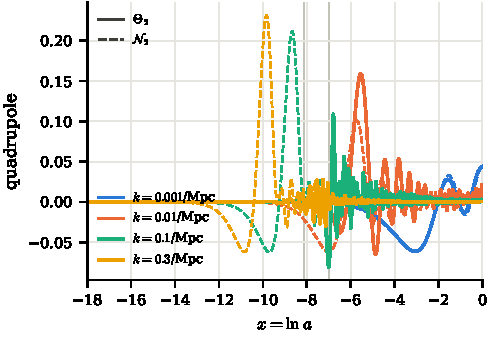
\includegraphics[width=\columnwidth]{m3_quadrupole}
\caption{Photon quadrupole $\Theta_2$ (solid) and neutrino quadrupole $\mathcal{N}_2$ (dashed).}
\label{fig:quadrupole}
\end{figure}

\begin{figure}
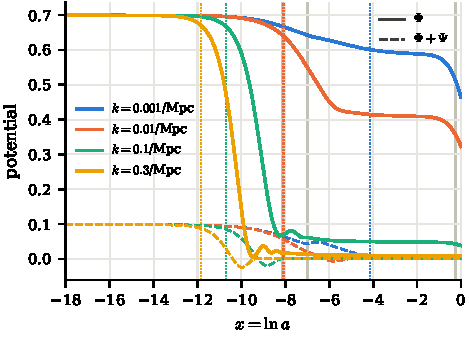
\includegraphics[width=\columnwidth]{m3_Phi}
\caption{Potentials $\Phi$ (solid) and $\Phi+\Psi$ (dashed). $\Phi+\Psi\neq0$ is the anisotropic stress of the
neutrinos, which is significant only during RD.}
\label{fig:Phi}
\end{figure}

\paragraph*{Quadrupoles.} The photon quadrupole (Fig.~\ref{fig:quadrupole}) is suppressed by scattering until
recombination, $\Theta_2\propto(\kappa/\tau')\Theta_1$: every scattering erases the anisotropy. As $|\tau'|$ falls
during recombination it grows rapidly, and after decoupling it reaches about a quarter of $\Theta_0$ as the photons
free-stream. The neutrino quadrupole is present from the start, since nothing isotropizes the neutrinos.

\paragraph*{Potentials.} Figure~\ref{fig:Phi} shows the potentials.
\begin{itemize}
\item $\Phi$ is constant outside the horizon. The neutrino anisotropic stress makes $\Phi+\Psi\neq0$: in RD
      $\Phi/\Psi=-(1+2f_\nu/5)$, a $16\%$ effect. As matter takes over, the neutrinos' share of the energy, and with it
      $\Phi+\Psi$, falls; it also decays once a mode is inside the horizon and the neutrinos have dispersed.
\item For modes that enter in RD, $\Phi$ decays and oscillates after horizon entry, as in the analytic solution.
      Radiation pressure keeps the photon density perturbation from growing while the background radiation density
      falls as $a^{-4}$, so the potential it sources decays as $a^{-2}$.
\item Once matter dominates, $\Phi$ is constant on all scales: the growing matter perturbation exactly compensates the
      dilution of the background. This is why $\Phi$ for $k=0.1$ and $0.3\Mpc^{-1}$ freezes at a small value after
      equality.
\item For $k=0.001\Mpc^{-1}$ we see the superhorizon transition from $0.699$ in RD to $0.586$ at $x=-1.5$, close to the
      MD value $3/5$; the ratio $0.84$ differs from $9/10$ because of the neutrinos.
\item When $\Lambda$ takes over, growth slows down and all potentials decay, by about $20\%$ today. This late decay is
      the source of the late ISW effect in the CMB.
\end{itemize}

\begin{figure*}
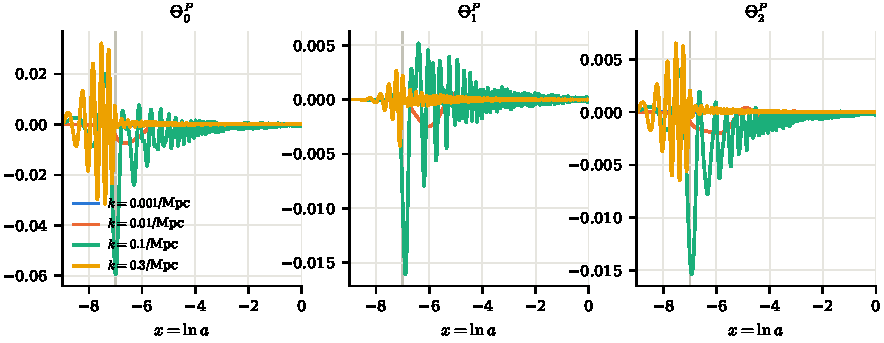
\includegraphics[width=\textwidth]{m3_polarization}
\caption{Polarization multipoles $\Theta^P_0$, $\Theta^P_1$ and $\Theta^P_2$ from shortly before decoupling (grey
line) until today.}
\label{fig:polarization}
\end{figure*}

\paragraph*{Polarization.} The polarization multipoles (Fig.~\ref{fig:polarization}) are generated only by Thomson
scattering of a quadrupole. Polarization therefore needs two things at once: scattering, and a quadrupole. Before
recombination the scattering is so efficient that the quadrupole is tiny, $\Theta_2\sim(\kappa/\tau')\Theta_1$. After
decoupling the quadrupole is large, but there is no more scattering. Polarization is produced only during the short
interval when the photons are starting to free-stream but still scattering occasionally, i.e.\ during the width of the
visibility function. Since $\Theta_2\propto\kappa\Theta_1$, the polarization traces the photon \emph{velocity}, not the
density, at last scattering. As a result:
\begin{itemize}
\item the $E$-mode signal is about a factor 10 weaker than the temperature signal;
\item it is very sensitive to the duration of recombination;
\item its acoustic peaks are out of phase with those of the temperature (Sec.~\ref{sec:m4}).
\end{itemize}
After decoupling the multipoles free-stream and decay. Reionization gives a small second burst at $x\approx-2$,
which is responsible for the low-$\ell$ $E$-mode bump.
